\documentclass{article}

\usepackage{../preamble}
\standalonetrue

\title{MATH 316 Lecture 10}
\author{Ashtan Mistal}
\date{May 27 2021}

\begin{document}

\ifstandalone
\maketitle
\fi

\graphicspath{{./Lecture10/}}

\section{Recap of Last Lecture}

Last class, we solved homogeneous heat / diffusion PDEs. We used the method of separation of variables, where we assumed $u(x,t)$ can be separated into two functions $X_x$ and $T_t$, such that $u(x,t) = X_x T_t$:

We then substituted that into the PDE, getting two equations; IVP and a BVP. We represented the solutions as a superposition of solutions for each eigenvalue and eigenfunction. 

We then found the coefficients of the Fourier series, or the series of the solution, by writing the initial condition in terms of Fourier series. 

Then we can match up the coefficients and match up the coefficients of the Fourier series into the solution that we found for the PDE. 

Today, we will continue to do more examples. 

\section{Examples}

\subsection{Example 4}

Note that these are the continued examples from the pdf file, named in last class. 1-3 are from last class also. 

$$\begin{matrix} u_t = 0.003 u_{xx} & 0 < x < 1; & t > 0 \end{matrix}$$

$$\begin{matrix} u_x (0,t) = u_x (1,t) = 0 & t > 0 \end{matrix} $$

$$\begin{matrix} u(x,0) = 50x (1-x) & 0 \leq x \leq 1 \end{matrix}$$

How long does it take for $u(0.5,t)$ to obtain its steady-state value, with 1\% error?

\hfill

\hrule

\hfill

The solution must be of this form: Note that this is a Neumann boundary condition. 
\begin{equation}
    u(x,t) = d_0 + \sum_{n = 1}^\infty \cos \left(\frac{n \pi x}{L} \right) e^{- \alpha \left( \frac{n \pi }{L} \right) ^2 t}
\end{equation}

Given that $\alpha = 0.003$, $L = 1$, and that $f(x) = 50x (1-x)$, we substitute:

We need to write the Fourier cosine series for $f(x)$:

$$a_0 = \frac{2}{1} \int_0^1 50x(1-x) dx = \left. 100 \left( \frac{x^2}{2} - \frac{x^3}{3} \right) \right|_0^1 = \frac{100}{6}$$

$$a_n = 2 \cdot 50 \int_0^1 x(1-x) \cos \left( \frac{n \pi x}{L} \right) dx = \left. \frac{100}{n \pi} x (1-x) \sin  \left( \frac{n \pi x}{1} \right) \right|_0^1 - \frac{100}{n \pi} \int_0^1 (1-2x) \sin (n \pi x) dx$$

$$a_n = \left. \frac{100}{(n \pi)^2} (1 - 2x) \cos(n \pi x) \right|_0^1 + \frac{200}{(n \pi)^2} \int_0^1 \cos(n \pi x) dx$$

$$a_n = \frac{100}{(n \pi)^2} \left( (-1)^{n+1} - 1 \right)$$

Hence:

$$f(x) = \frac{100}{6} + \sum_{n = 1}^\infty \frac{100}{(n \pi)^2} \left[(-1)^{n+1} - 1 \right] \cos(n \pi x)$$

$d_0 = \frac{50}{6}$ and $d_n = a_n$. This we substitute into (1) and simplify. 


$$u(x,t) = \frac{50}{6} + \frac{100}{\pi^2} \sum_{n = 1}^\infty \frac{\left[ (-1)^{n+1} - 1 \right]}{n^2} \cos(n \pi x) e^{- 0.003 (n \pi)^2 t}$$

As $t \to \infty$, $u(x,t) \to \frac{50}{6}$. This is the steady-state solution. This is also the mean value of the initial condition. (why?)

(n = 2)
\hfill

At $x - 0.5$: $u(x,t) - u(x,\infty) \approx \frac{50}{\pi} e^{-0.0012 \pi^2 t}$, which is $< \frac{1}{100} (\frac{50}{6})$

\hfill

If $0.0012 \pi^2 t > \ln(\frac{600}{\pi^2}) \Rightarrow t > \frac{1}{0.012 \pi^2} \ln \left( \frac{600}{\pi^2} \right) = 34.68 \text{s}$

The plot for the general solution is on the pdf file. 

\section{Inhomogeneous Equations}

In the previous examples, we solved heat / diffusion equations using separation of variables for homogeneous boundary conditions (Neumann and Dirichlet). Now, we are moving on to inhomogeneous equations. 

Either eq: $\frac{\partial u}{\partial t} = \alpha \frac{\partial^2 u}{\partial x^2} + g(x,t)$ or a boundary condition of $u(0,t) = a(t)$ (boundary condition is time dependent), or $u(L,t) = C \neq 0$. 

The idea is to solve these problems by decomposing it into a steady state problem and a homogeneous boundary condition problem, i.e. 

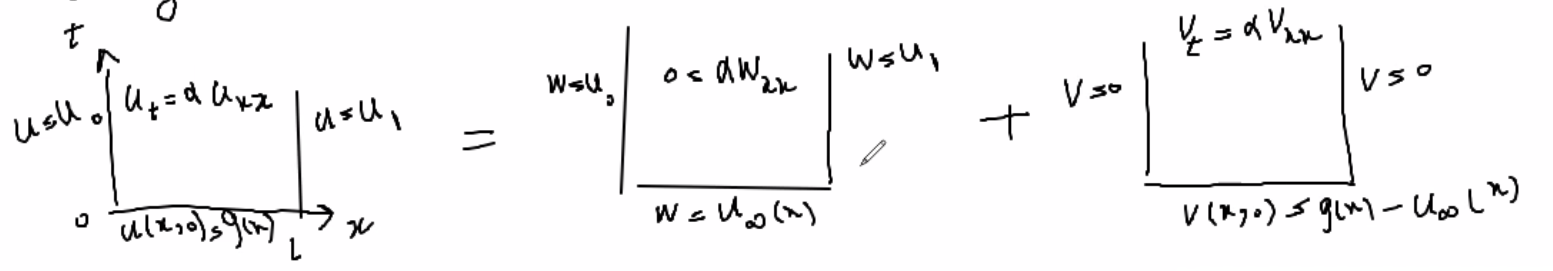
\includegraphics[width = 0.95 \textwidth]{image2.png}

Middle portion is the steady-state problem, and the right hand side is the transient problem with homogeneous boundary conditions. 

The general solution is thus:

$$u(x,t) = w(x) + v(x,t)$$

\subsection{Example 6}

$$\begin{matrix} u_t = \alpha u_{xx} & 0 < t < 1; & t > 0 \end{matrix}$$

$u(0,t) = 1$ and $u(1,t) = 3$ for $t > 0$ and $u(x,0) = x(1-x)$ for $0 \leq x \leq 1$

\subsubsection{Step 1}

We need to decompose the solution into two parts:

$$u(x,t) = \underbrace{u_s (x)}_{\text{Steady-state}} + \underbrace{v(x,t)}_{\text{Transient}}$$

\subsubsection{Step 2}

$$0 = \alpha \frac{\partial^2 u_s}{\partial x^2}$$

$u_s(0) = 1$ and $u_s(1) = 3$ $\rightarrow u_s = A x + B$

$u_s(0) = 1 \rightarrow B = 1$

$u_s(1) = 3 \rightarrow A = 2$

Therefore $u_s = 2 x + 1$

\subsubsection{Step 3}

Formulate $v(x,t)$ and find boundary conditions and initial conditions. 

Boundary conditions:

$v(0,t) = u(0,t) - u_s(0) = 0$

$v(1,t) = u(1,t) - u_s(1) = 0$

Initial conditions:

$$v(x,0) = u(x,0) - u_s(x) = x(1-x) - (2x+1) = -(x^2 + x + 1)$$

$$\frac{\partial u}{\partial t} = \frac{\partial}{\partial t} \left( u_s (x) + v(x,t) \right) = \frac{\partial v}{\partial t}$$

$$\alpha \frac{\partial^2 u}{\partial x^2} = \alpha \frac{\partial^2}{\partial x^2} \left( u_s (x) + v(x,t) \right) = \alpha \frac{\partial^2 v}{\partial x^2}$$

$$\Rightarrow \frac{\partial v}{\partial t} = \alpha \frac{\partial^2 v}{\partial x^2}$$

note: Similar to example 1 and 2, it is a standard (homogeneous) Dirichlet problem. 

\subsubsection{Step 4}

Solve the transient problem. 

$$v(x,t) = \sum_{n = 1}^\infty b_n \sin(n \pi x) e^{-\alpha (n \pi)^2 t}$$

(Refer to example 1 and 2)

$$b_n = \frac{-2}{1} \int_0^1 (1 + x + x^2) \sin(n \pi x) dx = \frac{2}{n \pi} \left[ 3(-1)^n - 1 \right] - \frac{4}{(n \pi)^3} \left[(-1)^n - 1 \right]$$

$$\Rightarrow v(x,t) = \sum_{n = 1}^\infty \left( \frac{2}{n \pi} \left[ 3(-1)^n - 1 \right] - \frac{4}{(n \pi)^3} \left[(-1)^n - 1 \right] \right) \sin(n \pi x) e^{-\alpha (n \pi)^2 t}$$

\subsubsection{Step 5}

Sum the steady state and transient parts of the solution. 

$$u(x,t) = u_x (x) + v(x,t)$$

$$u(x,t) = 1 + 2x + \sum_{n = 1}^\infty \left( \frac{2}{n \pi} \left[ 3(-1)^n - 1 \right] - \frac{4}{(n \pi)^3} \left[(-1)^n - 1 \right] \right) \sin(n \pi x) e^{-\alpha (n \pi)^2 t}$$

\subsection{Example 7}

Inhomogeneous equation and boundary conditions

Equation is given to be the heat equation:

$$\rho c_p \frac{\partial T}{\partial t} = k \frac{\partial^2 T}{\partial x^2} + Q(x)$$

$Q$ is a source (or sink) of heat. 

Let $p = 8940 \frac{kg}{m^3}$, $c_p = 914 \frac{J}{kg \cdot C}$, $k = 930 \frac{W}{m \cdot C}$ $L = 10 m$

Boundary conditions:

$$\begin{matrix} T(10,t) = 30 \\ T(0,t) = 30 \end{matrix}$$

Initial conditons:

$$T(x,0) = 30$$

$$Q(x) = 80000 x$$

Solution:

$$\frac{\partial T}{\partial t} = \alpha \frac{\partial^2 T}{\partial x^2} + q(x)$$

$$\alpha = \frac{k}{\rho c_p} \approx 10^{-4}$$

$$q(x) = \frac{Q(x)}{\rho c_p} = 0.01 x$$

We need to write $u = T(x,t)$

\subsubsection{Step 1}

We need to divide into two parts: 

$$u(x,t) = \underbrace{u_s (x)}_{\text{Steady-state}} + \underbrace{v(x,t)}_{\text{Transient}}$$

\subsubsection{Step 2}

$$0 = \alpha \frac{\partial^2 u_s}{\partial x^2} + q(x)$$

(note that the boundary conditions are $u_s(0) = 30 = u_s(10)$

$$\frac{\partial^2 u_s}{\partial x^2} + 100x = 0 \longrightarrow \frac{\partial u_s}{\partial x} + 50 x^2 = C_1$$

$$u_s = - \frac{50}{3} x^3 + C_1 x + C_2$$

Given boundary conditions: $u_s(0) = 30 \longrightarrow C_2 = 30$ and $u_s(10) = 30 \longrightarrow C_1 = \frac{10^4}{6}$

$$\Rightarrow u_s(x) = - \frac{50}{3} x^3 + \frac{10^4}{6} x = 30$$

\subsection{Step 3}

Formulate the transient part:

Boundary conditions:

$$\left\{ \begin{matrix} v(0,t) = u(0,t) - u_s(0) = 0 \\ v(10,t) = u(10,t) - u_s(10) = 0 \end{matrix} \right.$$

Initial conditions:

$$v(x,0) = 30 - u_s (x) = \frac{10^2}{6} x (x^2 - 100)$$

Double check these!!

Now, we need to solve for $v(x,t)$, which satisfies a standard Dirichlet problem. 

\subsubsection{Step 4}

$$v(x,t) = \sum_{n = 1}^\infty b_n \sin \left( \frac{n \pi}{10} x \right) e^{- 10^{-6} (n \pi)^2 t}$$

$$b_n = \frac{2}{10} \int_0^{10} \frac{10^2}{6} x (x^2 - 100) \sin( \frac{n \pi}{10} x) dx$$

\subsubsection{Step 5}

$$u(x,t) = u_s + v(x,t)$$

\end{document}
